% Usar el tipo de documento: Artículo científico.
\documentclass{beamer}

% Cargar mensajes en español.
\usepackage[spanish]{babel}

% Usar codificación utf-8 para acentos y otros.
\usepackage[utf8]{inputenc}

%Dimensiones de los márgenes.
%\usepackage[margin=1.5cm]{geometry}

% Insertar porciones de código
\usepackage{listings}

% Comenzar párrafos con separación no indentación.
\usepackage{parskip}
%enlaces
\usepackage{hyperref}
% Usar gráficos
\usepackage{graphicx}
\usepackage{caption}
\usepackage{subcaption}
%
% Usar contenedores flotantes para figuras.
\usepackage{float}

% Carpeta de las imágenes.
\graphicspath{{img/}}

% Configuración para porciones de código.
\lstset{
%	language=bash,
	basicstyle=\ttfamily\small,
%	numberstyle=\footnotesize,
%	numbers=left,
%	backgroundcolor=\color{gray!10},
%	frame=single,
	tabsize=4,
%	rulecolor=\color{black!30},
%	title=\lstname,
%	escapeinside={\%*}{*)},
	breaklines=true,
	breakatwhitespace=true,
%	framextopmargin=2pt,
%	framexbottommargin=2pt,
	extendedchars=false,
	inputencoding=utf8
}
%%%%%%%%%%%%%%%%%%%%%%%%%%%%%%%%%%%%%%%%%%%%%%%%%%%%%%%%%%%%%%%%%%%%%%%%%%%%%%%

% Propiedades
\title{Lenguaje de programación para cálculo paralelo.}

\author{Andrés Baamonde Lozano (andres.baamonde@udc.es)\\
	Rodrigo Arias Mallo (rodrigo.arias@udc.es)}

\begin{document}

%\maketitle

%%%%%%%%%%%%%%%%%%%%%%%%%%%%%%%%%%%%%%%%%%%%%%%%%%%%%%%%%%%%%%%%%%%%%%%%%%%%%%%
%\clearpage 

%\tableofcontents

%\clearpage 
\frame{\titlepage}
\begin{frame}
\frametitle{Introducción}
\begin{block}{Propósito}
\begin{itemize}
\item Lenguaje de programación orientado al cálculo numérico.
\item Objetivo: explotar al máximo la GPU y la CPU.
\end{itemize}
\end{block}
\pause
\begin{block}{Lenguajes relacionados}
\begin{itemize}
\item C, que implica una programación cuidadosa.
\item OpenCL, cuyo objetivo es ser un estándar abierto en el ámbito computación paralela.
\item Matlab, para las funciones sobre imágenes.
\end{itemize}
\end{block}
\end{frame}

\begin{frame}
\frametitle{Paradigma}
\begin{itemize}
\item Programación imperativa.
\item Necesaria sencillez para operar con la GPU.
\item Descartados otros paradigmas, no es necesario un alto nivel de abstracción.
\end{itemize}
\end{frame}

\begin{frame}
\frametitle{Gestión de memoria}
\begin{itemize}
\item A cargo del programador(como C).
\item Gestión de memoria dinámica retiene la memoria
más tiempo del necesario.
\end{itemize}
\end{frame}
\begin{frame}
\frametitle{Tipado}
\begin{itemize}
\item Tipado estático.
\item Se establece para las variables dimensión y tipo.
\item Incrementa el tiempo de desarrollo.
\item En tiempo de ejecución requiere menos comprobaciones.
\end{itemize}
\end{frame}
\begin{frame}
\frametitle{Tipos y modificadores}
\begin{block}{Tipos}
\begin{itemize}
\item Básico(C).
\item Complejos(Vector, Matriz,imaginario).
\end{itemize}
\end{block}
\pause
\begin{block}{Modificadores}
Además de los modificadores a nivel de función (Local) y a nivel de programa(Global).Existirán unos modificadores de tipos para cargar las variables en GPU o CPU.
\end{block}
\end{frame}
\begin{frame}
\frametitle{Operadores}
\begin{itemize}
\item Tradicionales de C.
\item Sobrecarga de operadores para los tipos complejos.
\end{itemize}
\end{frame}
\begin{frame}
\frametitle{Errores y características}
\begin{block}{Errores}
\begin{itemize}
\item Matemáticos.
\item Desbordamiento.
\item Segmentación.
\end{itemize}
\end{block}
\pause
\begin{block}{Características}
\begin{itemize}
\item Inserción de código OpenCL.
\item Evaluación en cortocircuíto.
\end{itemize}
\end{block}
\end{frame}
\begin{frame}
\frametitle{Las entrañas}

GPGPU =

General	Purpose computing on Graphics Processing Units

Usar la GPU como herramienta de computación

\pause

SIMD = Single Instruction, Multiple Data

Ejecutar una sóla instrucción a varios elementos a la vez.

\pause

OpenCL = Open Computing Language

Lenguaje para cálculo paralelo independiente del hw (2009).


\end{frame}



\begin{frame}
\frametitle{Rápida introducción a GPGPU en 3 pasos}

\begin{itemize}
\item Enviamos datos desde la RAM a la GPU.
\item La GPU realiza operaciones en su memoria interna.
\item Transferimos los datos de la GPU a la RAM.
\end{itemize}

Nota: La GPU tiene una memoria interna.

\end{frame}



\begin{frame}
\frametitle{Procesamiento paralelo}

\begin{itemize}
\item La GPU tiene muchos núcleos.
\item Pero sólo tiene una memoria.
\item Enviamos datos, y un programa común.
\item Cada núcleo ejecuta el mismo programa, con diferentes datos
\end{itemize}

\end{frame}


\begin{frame}
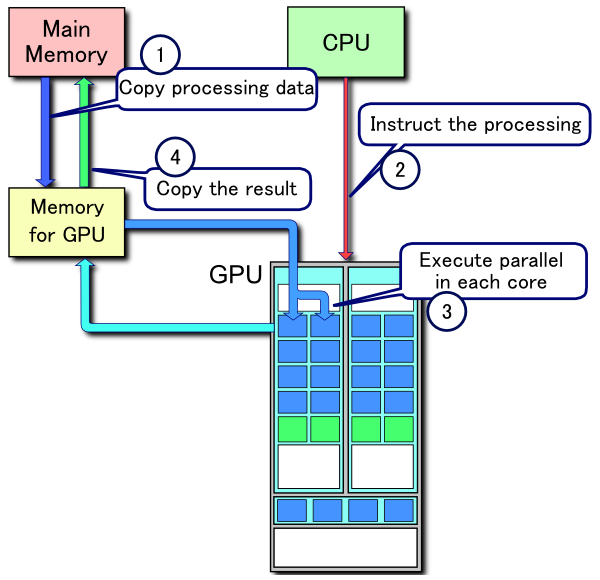
\includegraphics[width=\linewidth]{flow.png}
\end{frame}



\begin{frame}
\frametitle{Dónde está la mejora? Ejemplo de matrices.}

$A, B$ y $C$ son matrices de $NxN$. Disponemos de $P$ núcleos.

Calcular $C = A * B$. Complejidad $ O(n^3) $.


\begin{itemize}
\item Dividir la matriz $C$ en bloques de $P$ elementos.
\item Asignar cada elemento $(i,j)$ del bloque a un núcleo:
\item Repetir para todos los bloques.
\end{itemize}

\end{frame}



\begin{frame}
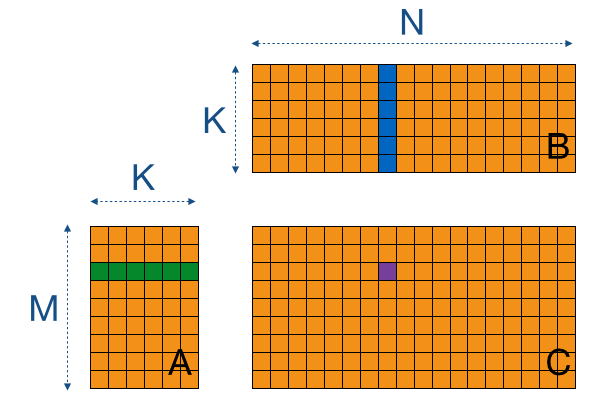
\includegraphics[width=\linewidth]{mat-mul.png}
\end{frame}



\begin{frame}[fragile]
Procesamiento paralelo, en cada núcleo

\begin{lstlisting}

    C[i][j] = 0;
    for(k = 0; k < K; k++)
        C[i][j] += A[i][k] * B[k][j];

\end{lstlisting}

Complejidad final de $ O(n^3 / P) $

\end{frame}



\begin{frame}
\frametitle{Demo}
Multiplicación de matrices.
\end{frame}



\begin{frame}
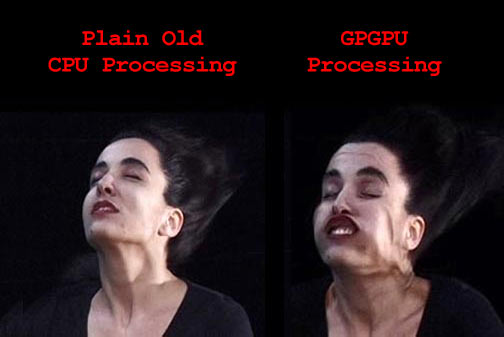
\includegraphics[width=\linewidth]{aire-cara.jpg}
\end{frame}



\begin{frame}

\frametitle{Ejemplo de filtro.}

Cada núcleo ejecuta un pequeño programa, como sumar los valores
de los píxeles vecinos.

El resultado se almacena en un lugar aparte, sin modificar la original.

Todos los núcleos se pueden ejecutar en paralelo.

La imagen resultante, regresa a la RAM.

\end{frame}



\begin{frame}
\center
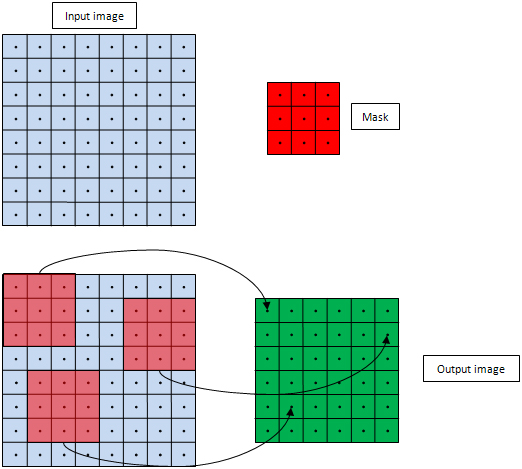
\includegraphics[width=\textheight]{convolucion.jpg}
\end{frame}



\begin{frame}
\frametitle{Problema}

Sabemos resolver muchos problemas, empleando algoritmos secuenciales.
Convertir un algoritmo a uno paralelo, requiere replantearlo.

\end{frame}



\begin{frame}[fragile]
\frametitle{Solución?}

Realizar cambios mecánicamente en el código secuencial para vectorizar aquello
que sea posible. Rama de investigación, vectorización.

Ejemplo:

\begin{lstlisting}
    for(i = 0; i < N; i++)
    {
        A[i]++;
        A[N-1-i]++;
    }
\end{lstlisting}

El optimizador debe ser capaz de deducir:

\begin{lstlisting}
A = A + 2;
\end{lstlisting}

\end{frame}



\begin{frame}
\frametitle{Optimización de código secuencial}
Tratar de paralelizar todo el código posible.

Crear un grafo de operaciones y simplificarlo.
\end{frame}



\begin{frame}[fragile]
Código de ejemplo

\begin{lstlisting}
 A = B*C + D*E
 C = A+E + E*B
 B = B*E + C
\end{lstlisting}

Descomposición:

\begin{lstlisting}
1    F = B*C
2    G = D*E
3    A = F+G
4    H = A*E
5    C = H+B
6    I = B*E
7    B = I*C
\end{lstlisting}

\end{frame}



\begin{frame}[fragile]
Descomposición:
\begin{lstlisting}
1    F = B*C
2    G = D*E
3    A = F+G
4    H = A*E
5    C = H+B
6    I = B*E
7    B = I*C
\end{lstlisting}
Tabla de operaciones:
\begin{lstlisting}
  A B C D E F G H I
  -----------------
1   . .     1      
2       . .   2        
3 3         . .        
4 .       .     4     
5   . 5         .
6   .     .       6
7   7 .           .
\end{lstlisting}
\end{frame}



\begin{frame}[fragile]
Tabla de operaciones:
\begin{lstlisting}
  A B C D E F G H I
  -----------------
1   . .     1      
2       . .   2        
3 3         . .        
4 .       .     4     
5   . 5         .
6   .     .       6
7   7 .           .
\end{lstlisting}
Optimización de operaciones.
\begin{lstlisting}
  A B C D E F G H I
  -----------------
1   . . . . 1 2    
2 3         . .       
3 .       .     4    
4   . 5   .     . 6
5   7 .           .
\end{lstlisting}
\end{frame}



\begin{frame}[fragile]
Optimización de operaciones.
\begin{lstlisting}
  A B C D E F G H I
  -----------------
1   . . . . 1 2    
2 3         . .       
3 .       .     4    
4   . 5   .     . 6
5   7 .           .
\end{lstlisting}
Optimización del espacio.
\begin{lstlisting}

  A B C D E F G H I
  -----------------
1   . . . . 1 2    
2 3         . .    
3 .       . 4      
4   . 5   . . 6    
5   7 .       .    
\end{lstlisting}
\end{frame}



\begin{frame}

\end{frame}



\begin{frame}
\center ¿Preguntas?
\end{frame}

\end{document}
